\documentclass{article}

\usepackage[T1]{fontenc}
\usepackage[utf8]{inputenc}
\usepackage[greek,english]{babel}
\usepackage[a4paper, margin=0.2in]{geometry}
\usepackage{CJKutf8}

\usepackage{float}
\usepackage{graphicx}

\begin{document}
\begin{CJK}{UTF8}{gbsn}

\title{hw5}
\author{刘本嵩 U201614531}

\maketitle

% \foreignlanguage{greek}{φΔδ} \begin{CJK}{UTF8}{gbsn}汉\end{CJK}

\section{Q9.9}
\Large
\smallskip

(1)

    $$Cube_2(12) = 12 xor bin(0100) = 8$$
    $$\sigma(8) = 8<<1 = 16$$
    $$\beta(9) = 24$$
    $$PM2I_{+3}(28) = (28+8) mod 32 = 4$$
    $$Cube_0(\sigma(4)) = 8+1 = 9$$
    $$\sigma(Cube_0(18)) = (uint5_t)19<<1 = 7$$

(2) 网络直径为$2n-1=9$,由bin(00101)到bin(00111),依次经过6步:

    00101 -> 01010 -> 10100 -> 01001 -> 10010 -> 10011 -> 00111

(3) 网络直径为3, 结点度为9, 与2号距离最远的是13, 15, 21, 23。

\section{Q9.13}
\Large
\smallskip

能.

\begin{figure}[H]
\centering
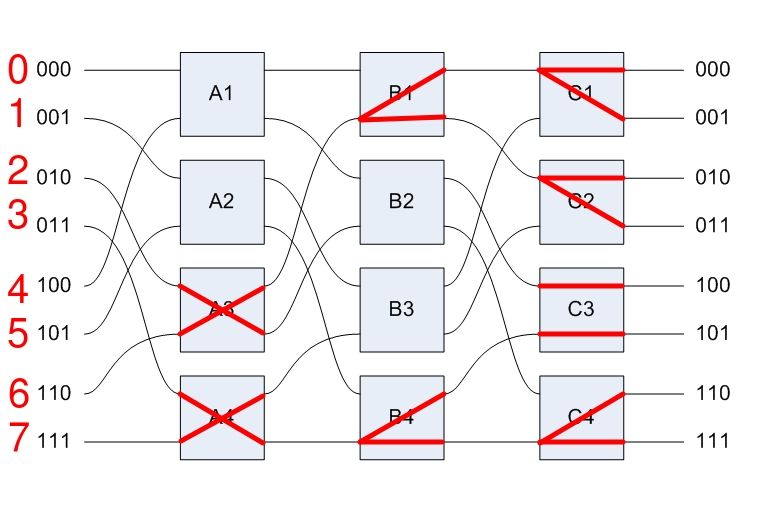
\includegraphics[scale=0.5]{hw5-img1.jpg}
\caption{开关状态图} 
\end{figure}


\end{CJK}
\end{document}

